\documentclass[11pt,letterpaper]{article}
\usepackage[margin=1in]{geometry}
\usepackage{booktabs}
\usepackage{amsmath}
\usepackage{graphicx}
\usepackage{xcolor}
\usepackage{hyperref}
\usepackage{fancyhdr}
\usepackage{float}
\usepackage{caption}
\usepackage{enumitem}
\usepackage{longtable}

\definecolor{gain}{RGB}{0,128,0}
\definecolor{loss}{RGB}{200,0,0}
\definecolor{neutral}{RGB}{80,80,80}

\pagestyle{fancy}
\fancyhf{}
\rhead{Allocation Engine --- Internal}
\lhead{YTD Performance Report}
\rfoot{\thepage}

\title{%
  \textbf{YTD Performance Report} \\[4pt]
  \large Allocation Engine: March 2--25, 2026 \\[2pt]
  \normalsize Data sourced from Netlify blob store (market-quotes \& options-chain)
}
\author{Allocation Engine Research}
\date{March 25, 2026}

\begin{document}
\maketitle
\thispagestyle{fancy}

% ============================================================
\section{Executive Summary}
% ============================================================

This report summarises the allocation engine's YTD performance using
daily market data captured in the Netlify blob store from
\textbf{March~2--25, 2026} (24 trading days).

\begin{table}[H]
\centering
\caption{YTD performance summary}
\begin{tabular}{lr}
\toprule
Metric & Value \\
\midrule
BTC/USD return (Mar~2--25)   & \textcolor{gain}{+4.9\%} \\
BTC share return (Mar~2--25) & \textcolor{gain}{+5.9\%} \\
BTC/USD annualised vol       & 39.4\% \\
BTC/USD high / low           & \$74,554 / \$66,452 \\
BTC share high / low         & \$32.93 / \$30.09 \\
BTC/USD max drawdown         & \textcolor{loss}{-8.8\%} \\
\midrule
IWN ATM IV (period avg)      & 29.5\% \\
IWN ATM IV high / low        & 34.8\% / 24.1\% \\
\midrule
BTC trading P\&L (Feb~21--Mar~4) & \textcolor{gain}{+\$15,770} \\
Options P\&L (Feb~21--Mar~4) & \textcolor{gain}{+\$4,195} \\
\textbf{Total engine P\&L} & \textcolor{gain}{\textbf{+\$19,965}} \\
\bottomrule
\end{tabular}
\end{table}

% ============================================================
\section{Daily Market Data}
% ============================================================

\begin{figure}[H]
  \centering
  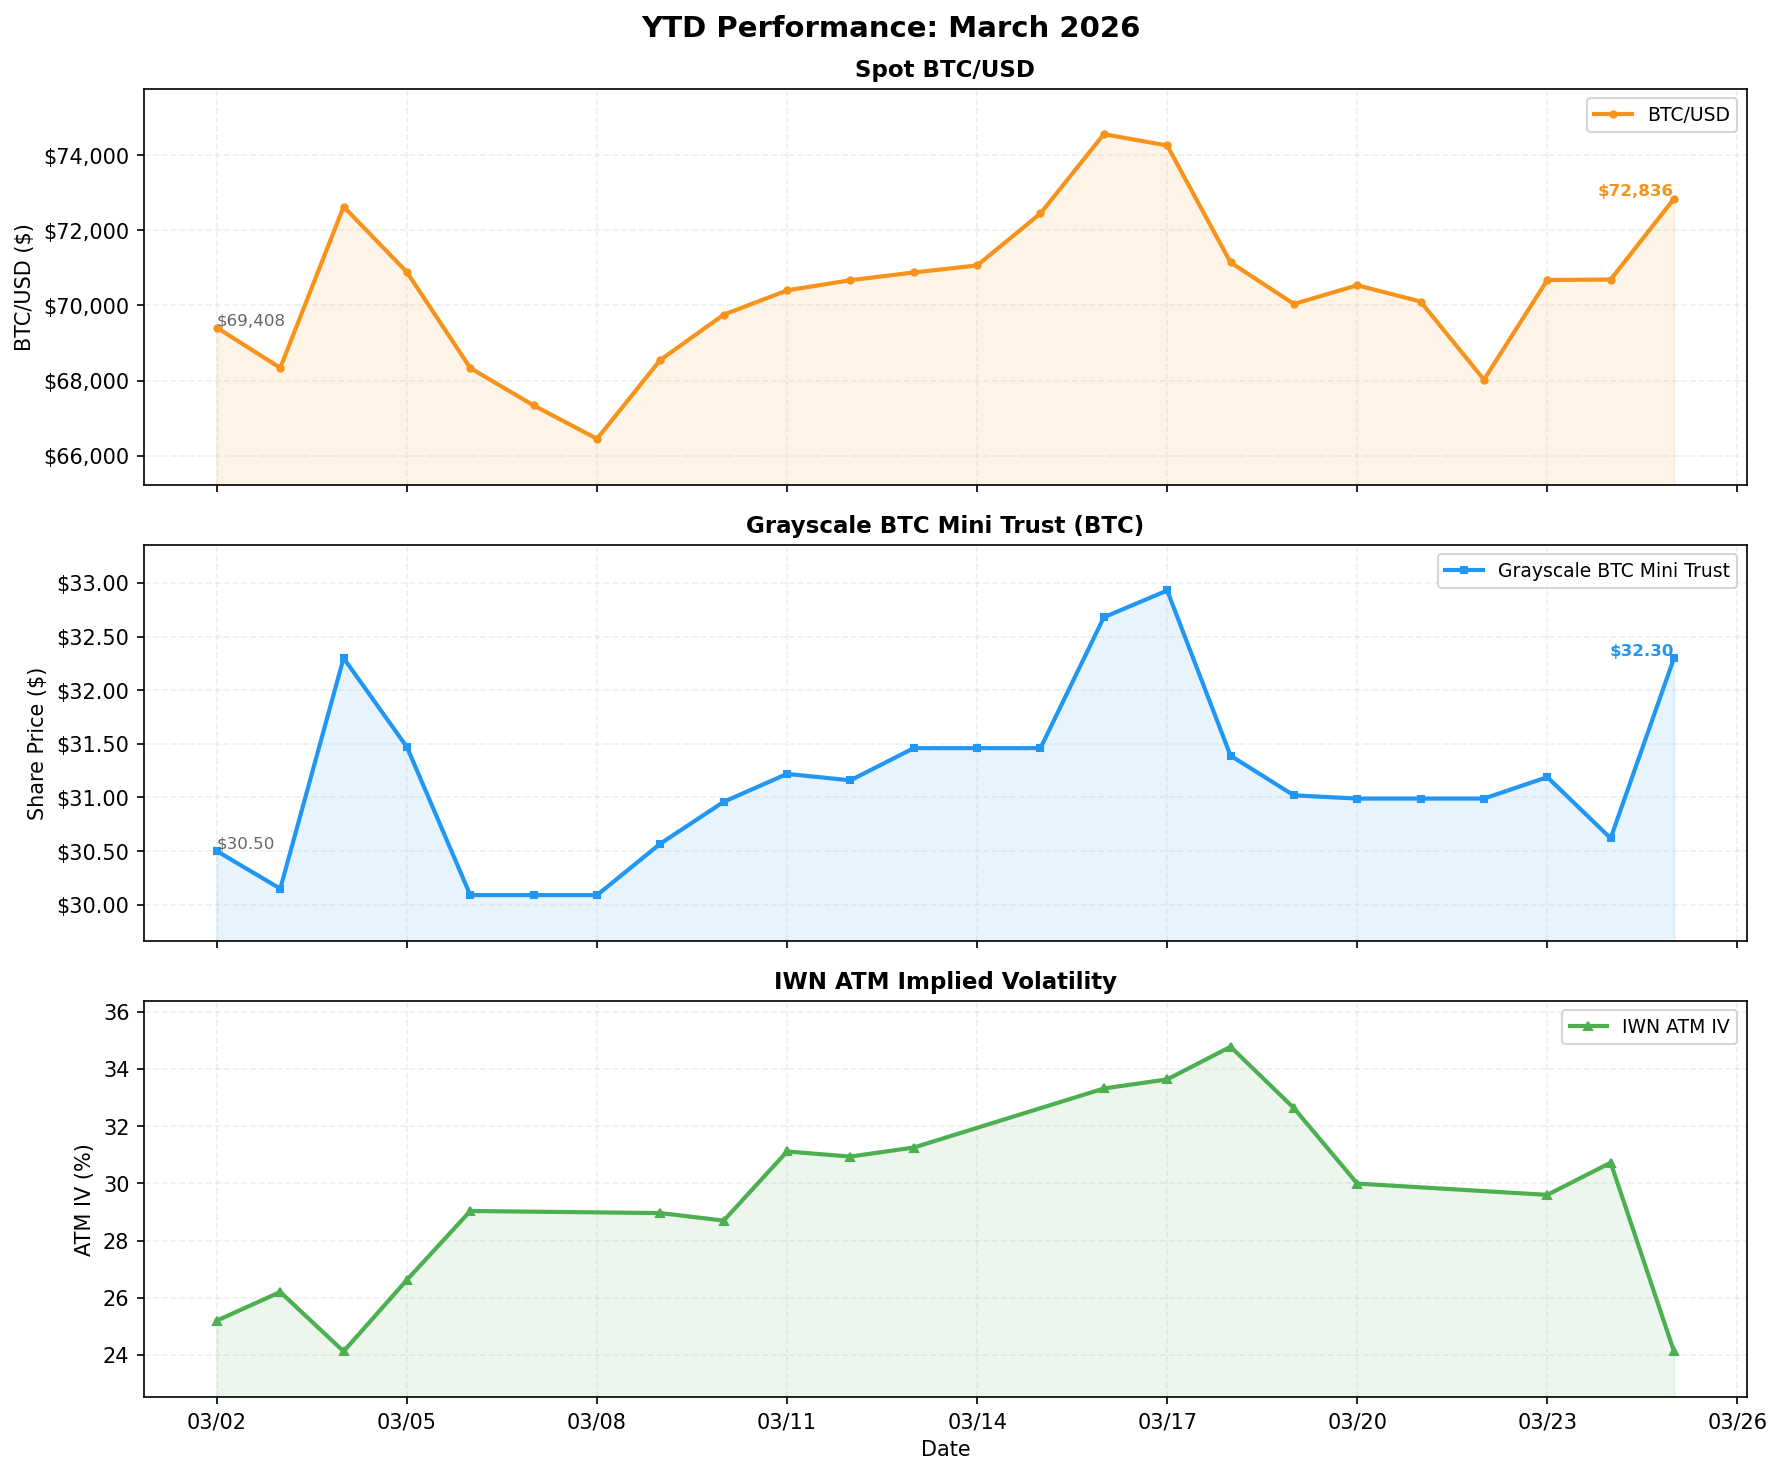
\includegraphics[width=\textwidth]{ytd_performance.png}
  \caption{YTD price action: BTC/USD (top), Grayscale BTC Mini Trust share
  price (middle), and IWN ATM implied volatility (bottom). Data from
  Netlify blob store market-quotes and options-chain stores.}
\end{figure}

\begin{table}[H]
\centering
\caption{Daily prices and IWN ATM IV (from blob store)}
{\small
\begin{tabular}{l r r r}
\toprule
Date & BTC/USD & BTC Share & IWN ATM IV \\
\midrule
2026-03-02 & \$69,408 & \$30.50 & 25.2\% \\
2026-03-03 & \$68,339 & \$30.15 & 26.2\% \\
2026-03-04 & \$72,625 & \$32.30 & 24.1\% \\
2026-03-05 & \$70,884 & \$31.47 & 26.6\% \\
2026-03-06 & \$68,334 & \$30.09 & 29.0\% \\
2026-03-07 & \$67,340 & \$30.09 & --- \\
2026-03-08 & \$66,452 & \$30.09 & --- \\
2026-03-09 & \$68,551 & \$30.57 & 29.0\% \\
2026-03-10 & \$69,754 & \$30.96 & 28.7\% \\
2026-03-11 & \$70,399 & \$31.22 & 31.1\% \\
2026-03-12 & \$70,670 & \$31.16 & 30.9\% \\
2026-03-13 & \$70,876 & \$31.46 & 31.3\% \\
2026-03-14 & \$71,063 & \$31.46 & --- \\
2026-03-15 & \$72,446 & \$31.46 & --- \\
2026-03-16 & \$74,554 & \$32.68 & 33.3\% \\
2026-03-17 & \$74,253 & \$32.93 & 33.6\% \\
2026-03-18 & \$71,143 & \$31.39 & 34.8\% \\
2026-03-19 & \$70,038 & \$31.02 & 32.6\% \\
2026-03-20 & \$70,536 & \$30.99 & 30.0\% \\
2026-03-21 & \$70,102 & \$30.99 & --- \\
2026-03-22 & \$68,025 & \$30.99 & --- \\
2026-03-23 & \$70,676 & \$31.19 & 29.6\% \\
2026-03-24 & \$70,688 & \$30.62 & 30.7\% \\
2026-03-25 & \$72,836 & \$32.30 & 24.1\% \\
\bottomrule
\end{tabular}}
\end{table}

% ============================================================
\section{Realised P\&L}
% ============================================================

\subsection{BTC Trading (Feb 21 -- Mar 4)}

The engine executed a bracket strategy on Grayscale BTC Mini Trust,
buying 1,575 shares at an average of \$29.76 and selling 2,054 shares
at an average of \$30.50, generating \textcolor{gain}{+\$15,770} in
trading P\&L on round-trip volume.

\subsection{Options Round-Trips}

\begin{table}[H]
\centering
\caption{Closed options round-trips (Feb 21 -- Mar 4, 2026)}
{\small
\begin{tabular*}{\textwidth}{@{\extracolsep{\fill}}l r l r r r r}
\toprule
Contract & Qty & Dates & Open & Close & P\&L & Return \\
\midrule
IWM \$262 Put 3/11 & 10 & 02/26 $\to$ 02/27 & \$3.16 & \$4.96 & \textcolor{gain}{+\$1,800} & +57\% \\
IWM \$247 Put 3/13 & 10 & 02/27 $\to$ 03/01 & \$1.41 & \$2.86 & \textcolor{gain}{+\$1,450} & +103\% \\
CRWD \$390 Put 3/06 & 1 & 02/25 $\to$ 02/27 & \$21.05 & \$33.30 & \textcolor{gain}{+\$1,225} & +58\% \\
CRWD \$367.5 Put 3/20 & 1 & 02/27 $\to$ 03/04 & \$19.05 & \$16.25 & \textcolor{loss}{--\$280} & --15\% \\
\midrule
\multicolumn{5}{l}{\textbf{Total Options P\&L}} & \textcolor{gain}{\textbf{+\$4,195}} & \\
\bottomrule
\end{tabular*}}
\end{table}

\subsection{Combined P\&L}

\begin{table}[H]
\centering
\caption{Combined engine P\&L summary}
\begin{tabular}{lr}
\toprule
Source & P\&L \\
\midrule
BTC bracket trading     & \textcolor{gain}{+\$15,770} \\
IWM put round-trips     & \textcolor{gain}{+\$3,250} \\
CRWD put round-trips    & \textcolor{gain}{+\$945} \\
\midrule
\textbf{Total}        & \textcolor{gain}{\textbf{+\$19,965}} \\
\bottomrule
\end{tabular}
\end{table}

% ============================================================
\section{Volatility Environment}
% ============================================================

The IWN ATM implied volatility averaged \textbf{29.5\%} over
the period, ranging from 24.1\% to 34.8\%. This level is
consistent with the 21-day realised vol of 18.4\% reported in the main
strategy document, suggesting options are \textbf{fairly priced} relative
to realised moves.

Key observations:
\begin{itemize}[nosep]
  \item BTC/USD traded in a \$66,452--\$74,554 range
        (+4.9\% net) with 39\% annualised vol
  \item Grayscale BTC share tracked spot with +5.9\% return
        vs +4.9\% for spot BTC/USD
  \item IWN IV remained stable, supporting continued use of the put
        hedging strategy at current pricing levels
  \item The maximum intra-period BTC/USD drawdown was
        \textcolor{loss}{-8.8\%}, highlighting the need for
        the correlated put hedge overlay
\end{itemize}

\end{document}
